\section{Computational model}

        Il modello migliore è stato ottenuto dopo una prima fase di \textit{data preparation}, ed una successiva fase di \textit{hyper-parameter tuning}.

        \subsection{Data preparation}
        
                \subsubsection{Data splitting}
                
                        Il \textit{dataset} è stato diviso in due sezioni differenti:
                        \begin{itemize}
                                \item \textit{training set}: contiene 80\% dell'intero dataset originale (6400 records)
                                \item \textit{test set}: contiene il restante 20\% del dataset originale (1600 records)
                        \end{itemize}
                
                \subsubsection{Bad values management}
                
                        Il \textit{dataset} originale (\textit{training\_set.csv}) contiene dati mancanti in corrispondenza di alcune delle \textit{features}, per questo motivo, i valori relativi a tali campi sono stati sostituiti con la mediana relativa alla colonna della \textit{feature} corrispondente all'interno del \textit{dataset}.
                        \bigbreak
                        
                        In seguito, sono stati analizzati gli \textit{outliers}. Un \textit{outlier} è un'osservazione che devia marcatamente da altre osservazioni nel campione di dati. L'identificazione di potenziali \textit{outliers} è importante dal momento che potrebbero indicare dati corrotti o mal codificati, anche se, in alcuni casi, potrebbero essere il risultato di variazioni casuali nel campione di dati.
                        
                        L'individuazione degli \textit{outliers} dipende dalla distribuzione dei dati sottostante. Il \textit{dataset} considerato, come si evince dal pair-plot in figura \ref{fig:training_set_pairplot}, segua approssimativamente una distribuzione \textit{Normale}, pertanto sono stati analizzati i risultati derivanti da tre metodi:
                        \begin{itemize}
                            \item \textit{z-score}
                            \item \textit{modified z-score}
                            \item \textit{inter-quartile range}
                        \end{itemize}
                    
                        Lo \textit{Z-score} di una osservazione è definito come:
                        \begin{displaymath}
                                z_i = \frac{x_i - \mu_x}{\sigma_x}
                        \end{displaymath}
                        essendo $\mu_x$ e $\sigma_x$, rispettivamente, la media e la deviazione standard del campione di dati. Sono considerati \textit{outliers} i campioni con il valore assoluto dello score maggiore di $3$.
                        \smallbreak
                        
                        Lo \textit{Z-score modificato} (\textit{Iglewicz and Hoaglin}) è definito come:
                        \begin{displaymath}
                                m_i = \frac{0.6745 \cdot (x_i - \tilde{x})}{MAD}
                        \end{displaymath}
                        essendo $MAD$ la median absolute deviation e $\tilde{x}$ la mediana. Sono considerati \textit{outliers} i campioni con il valore assoluto dello score maggiore di $3.5$.
                        \smallbreak
                        
                        L'\textit{inter-quartile range} è definito come:
                        \begin{displaymath}
                                IQR = Q_3 - Q_1
                        \end{displaymath}
                        essendo $Q_1$ e $Q_3$, rispettivamente, il primo ed il terzo quartile del campione di dati. Sono considerati \textit{outliers} i campioni con uno valore maggiore di $Q_3 + IQR \cdot 1.5$ e minore di $Q_1 - IQR \cdot 1.5$.
                        \smallbreak
                        
                        Per non ridurre la numerosità del \textit{training set} si è scelto di sostituire (e non eliminare) gli \textit{outliers} con la mediana relativa ad una determinata \textit{feature}. Si è ritenuto opportuno utilizzare la mediana in quanto è una misura più robusta per la rappresentazione della dispersione di valori rispetto alla media essendo meno soggetta alla presenza di \textit{outliers}.                        
                
                \subsubsection{Data normalization}
                
                La normalizzazione è il processo di ridimensionamento dei singoli campioni per avere una norma unitaria. Questo processo può essere utile se si prevede di utilizzare una forma quadratica come il prodotto scalare o qualsiasi altro kernel per quantificare la somiglianza di qualsiasi coppia di campioni.Per effettuare la normalizzazione dei campioni sono stati utilizzati gli scalers: \textit{MinMaxScaler, MaxAbsScaler, QuantileTransformer (uniform output), PowerTransformer (Yeo-Johnson e Box-Cox transforms)}.
                
        		
        		\begin{center}
        			La tabella \ref{tab:fscoreMLMinMax} mostra i risultati ottenuti con MinMaxScaler\\
                \begin{tabular}{+l^c^c}
                	\toprule\rowstyle{\bfseries}
                	Model & Parameters & F1-score \\
                	\toprule
                	
                	Multi-Layer Perceptron & \makecell[l]{activation: relu \\ hidden\_layer\_sizes: (100, 50) \\ learning\_rate: adaptive \\ learning\_rate\_init: 0.01 \\ solver: sgd} & \textbf{0.886} \\
                	\midrule
                	Support Vector Machine & \makecell[l]{C: 10 \\ decision\_function\_shape: ovo \\ gamma: 10 \\ kernel: rbf} & 0.794 \\
                	\midrule
                	Decision Tree & \makecell[l]{criterion: entropy \\ max\_depth: 90 \\ max\_features: None \\ min\_samples\_leaf: 1 \\ min\_samples\_split: 2 \\ splitter: best} & 0.607 \\
                	\midrule
                	Random Forest & \makecell[l]{criterion: entropy \\ max\_depth: 90 \\ max\_features: log2 \\ min\_samples\_leaf: 2 \\ min\_samples\_split: 2 \\ n\_estimators: 400} & 0.808 \\
                	\midrule
                	K-Nearest Neighbors & \makecell[l]{metric: minkowski \\ n\_neighbors: 3 \\ p: 4} & 0.768 \\
                	\midrule
                	Ada Boost &  \makecell[l]{class\_weight: balanced \\ max\_depth: 90 \\ max\_features: 3 \\ min\_samples\_leaf: 4 \\ n\_estimators: 400} & 0.823 \\
                	\midrule
                	Naive Bayes & \makecell[l]{priors: None \\ var\_smoothing: 10e-08} & 0.55 \\
                	\midrule
                	K-Means & \makecell[l]{max\_iter: 10000 \\ n\_clusters: 4 \\ random\_state: 43531} & 0.344 \\
                	
                	\toprule\rowstyle{\bfseries}
                \end{tabular}
                            \captionof{table}{\textit{F1-score} con sampler SMOTE e scaler MinMaxScaler}
            	\label{tab:fscoreMLMinMax}
		        \end{center}
	        
	        
	        
		        \begin{center}
		        	La tabella \ref{tab:f1scoreMLmaxAbs} mostra i risultati ottenuti con MaxAbsScaler\\
		        	\begin{tabular}{+l^c^c}
		        		\toprule\rowstyle{\bfseries}
		        		Model & Parameters & F1-score \\
		        		\toprule
		        		
		        		Multi-Layer Perceptron & \makecell[l]{activation: relu \\ hidden\_layer\_sizes: (150, 100) \\ learning\_rate: adaptive \\ learning\_rate\_init: 0.1 \\ solver: sgd} & \textbf{0.84} \\
		        		\midrule
		        		Support Vector Machine & \makecell[l]{C: 10 \\ decision\_function\_shape: ovo \\ gamma: 10 \\ kernel: rbf} & 0.692 \\
		        		\midrule
		        		Decision Tree & \makecell[l]{criterion: entropy \\ max\_depth: 90 \\ max\_features: None \\ min\_samples\_leaf: 1 \\ min\_samples\_split: 2} & 0.625 \\
		        		\midrule
		        		Random Forest & \makecell[l]{criterion: entropy \\ max\_depth: 80 \\ max\_features: sqrt \\ min\_samples\_leaf: 2 \\ min\_samples\_split: 2 \\ n\_estimators: 400} & 0.813 \\
		        		\midrule
		        		K-Nearest Neighbors & \makecell[l]{metric: minkowski \\ n\_neighbors: 3 \\ p: 3} & 0.76 \\
		        		\midrule
		        		Ada Boost &  \makecell[l]{class\_weight: balanced \\ max\_depth: 90 \\ max\_features: 3 \\ min\_samples\_leaf: 4 \\ n\_estimators: 300} & 0.815 \\
		        		\midrule
		        		Naive Bayes & \makecell[l]{priors: None \\ var\_smoothing: 0.01} & 0.549 \\
		        		\midrule
		        		
		        		\toprule\rowstyle{\bfseries}
		        	\end{tabular}
	        	\captionof{table}{\textit{F1-score} con sampler SMOTE e scaler MaxAbsScaler}
	        	\label{tab:f1scoreMLmaxAbs}
		        \end{center}
	        
	        
	        
		        \begin{center}
		        	La tabella \ref{tab:f1scoreMLQuantile} mostra i risultati ottenuti con QuantileTransformer\\
		        	\begin{tabular}{+l^c^c}
		        		\toprule\rowstyle{\bfseries}
		        		Model & Parameters & F1-score \\
		        		\toprule
		        		
		        		Multi-Layer Perceptron & \makecell[l]{activation: relu \\ hidden\_layer\_sizes: (150, 100) \\ learning\_rate: adaptive \\ learning\_rate\_init: 0.1 \\ solver: sgd} & \textbf{0.828} \\
		        		\midrule
		        		Support Vector Machine & \makecell[l]{C: 10 \\ decision\_function\_shape: ovo \\ gamma: 10 \\ kernel: rbf} & 0.743 \\
		        		\midrule
		        		Decision Tree & \makecell[l]{criterion: entropy \\ max\_depth: 90 \\ max\_features: None \\ min\_samples\_leaf: 5 \\ min\_samples\_split: 2} & 0.616 \\
		        		\midrule
		        		Random Forest & \makecell[l]{criterion: entropy \\ max\_depth: 80 \\ max\_features: log2 \\ min\_samples\_leaf: 2 \\ min\_samples\_split: 2 \\ n\_estimators: 500} & 0.813 \\
		        		\midrule
		        		K-Nearest Neighbors & \makecell[l]{metric: minkowski \\ n\_neighbors: 11 \\ p: 3} & 0.809 \\
		        		\midrule
		        		Ada Boost &  \makecell[l]{class\_weight: balanced \\ max\_depth: 90 \\ max\_features: 3 \\ min\_samples\_leaf: 4 \\ n\_estimators: 200} & 0.818 \\
		        		\midrule
		        		Naive Bayes & \makecell[l]{priors: None \\ var\_smoothing: 0.01} & 0.492 \\
		        		\midrule
		        		
		        		\toprule\rowstyle{\bfseries}
		        	\end{tabular}
	        		        	\captionof{table}{\textit{F1-score} con sampler SMOTE e scaler QuantileTransformer}
	        	\label{tab:f1scoreMLQuantile}
		        \end{center}
	        
	        
	       
				 \begin{center}
					La tabella \ref{tab:f1scoreMLPowerTransformerYJ} mostra i risultati ottenuti con PowerTransformer (Yeo-Johnson)\\
					\begin{tabular}{+l^c^c}
						\toprule\rowstyle{\bfseries}
						Model & Parameters & F1-score \\
						\toprule
						
						Multi-Layer Perceptron & \makecell[l]{activation: relu \\ hidden\_layer\_sizes: (150, 100) \\ learning\_rate: adaptive \\ learning\_rate\_init: 0.1 \\ solver: sgd} & \textbf{0.821} \\
						\midrule
						Support Vector Machine & \makecell[l]{C: 50 \\ decision\_function\_shape: ovo \\ gamma: 10 \\ kernel: rbf} & 0.78 \\
						\midrule
						Decision Tree & \makecell[l]{criterion: entropy \\ max\_depth: 80 \\ max\_features: None \\ min\_samples\_leaf: 2 \\ min\_samples\_split: 2} & 0.616 \\
						\midrule
						Random Forest & \makecell[l]{criterion: entropy \\ max\_depth: 90 \\ max\_features: sqrt \\ min\_samples\_leaf: 2 \\ min\_samples\_split: 2 \\ n\_estimators: 200} & 0.813 \\
						\midrule
						K-Nearest Neighbors & \makecell[l]{metric: minkowski \\ n\_neighbors: 3 \\ p: 3} & 0.767 \\
						\midrule
						Ada Boost &  \makecell[l]{class\_weight: balanced \\ max\_depth: 90 \\ max\_features: 3 \\ min\_samples\_leaf: 4 \\ n\_estimators: 200} & 0.829 \\
						\midrule
						Naive Bayes & \makecell[l]{priors: None \\ var\_smoothing: 1e-08} & 0.553 \\
						\midrule
						
						\toprule\rowstyle{\bfseries}
					\end{tabular}
       		        	\captionof{table}{\textit{F1-score} con sampler SMOTE e scaler PowerTransformer (Yeo-Johnson)}
						\label{tab:f1scoreMLPowerTransformerYJ}
				\end{center}
        
        
        
        				 \begin{center}
			        	La tabella \ref{tab:f1scoreMLPowerTransformerBC} mostra i risultati ottenuti con PowerTransformer (Box-Box)\\
			        	\begin{tabular}{+l^c^c}
			        		\toprule\rowstyle{\bfseries}
			        		Model & Parameters & F1-score \\
			        		\toprule
			        		
			        		Multi-Layer Perceptron & \makecell[l]{activation: relu \\ hidden\_layer\_sizes: (150, 100) \\ learning\_rate: adaptive \\ learning\_rate\_init: 0.1 \\ solver: sgd} & \textbf{0.882} \\
			        		\midrule
			        		Support Vector Machine & \makecell[l]{C: 50 \\ decision\_function\_shape: ovo \\ gamma: 10 \\ kernel: rbf} & 0.78 \\
			        		\midrule
			        		Decision Tree & \makecell[l]{criterion: entropy \\ max\_depth: 80 \\ max\_features: None \\ min\_samples\_leaf: 2 \\ min\_samples\_split: 2} & 0.622 \\
			        		\midrule
			        		Random Forest & \makecell[l]{criterion: entropy \\ max\_depth: 80 \\ max\_features: log2 \\ min\_samples\_leaf: 2 \\ min\_samples\_split: 2 \\ n\_estimators: 400} & 0.812 \\
			        		\midrule
			        		K-Nearest Neighbors & \makecell[l]{metric: minkowski \\ n\_neighbors: 3 \\ p: 3} & 0.767 \\
			        		\midrule
			        		Ada Boost &  \makecell[l]{class\_weight: balanced \\ max\_depth: 90 \\ max\_features: 3 \\ min\_samples\_leaf: 4 \\ n\_estimators: 300} & 0.824 \\
			        		\midrule
			        		Naive Bayes & \makecell[l]{priors: None \\ var\_smoothing: 1e-08} & 0.553 \\
			        		\midrule
			        		
			        		\toprule\rowstyle{\bfseries}
			        	\end{tabular}
			        	\captionof{table}{\textit{F1-score} con sampler SMOTE e scaler PowerTransformer (Box-Cox)}
			        	\label{tab:f1scoreMLPowerTransformerBC}
			        \end{center}
        
                
                \subsubsection{Feature selection}
                
                        In questa fase sono state selezionate le \textit{features} più significative al fine di ridurre i costi di training e migliorare la capacità di generalizzazione del classificatore.
                        Per "filtrare" le features viene assegnato un punteggio ad ogni feature utilizzando una funzione infine vengono rimosse tutte tranne le k feature con il punteggio maggiore.
                   
                        
                        \begin{figure}[!h]
                            \centering
                            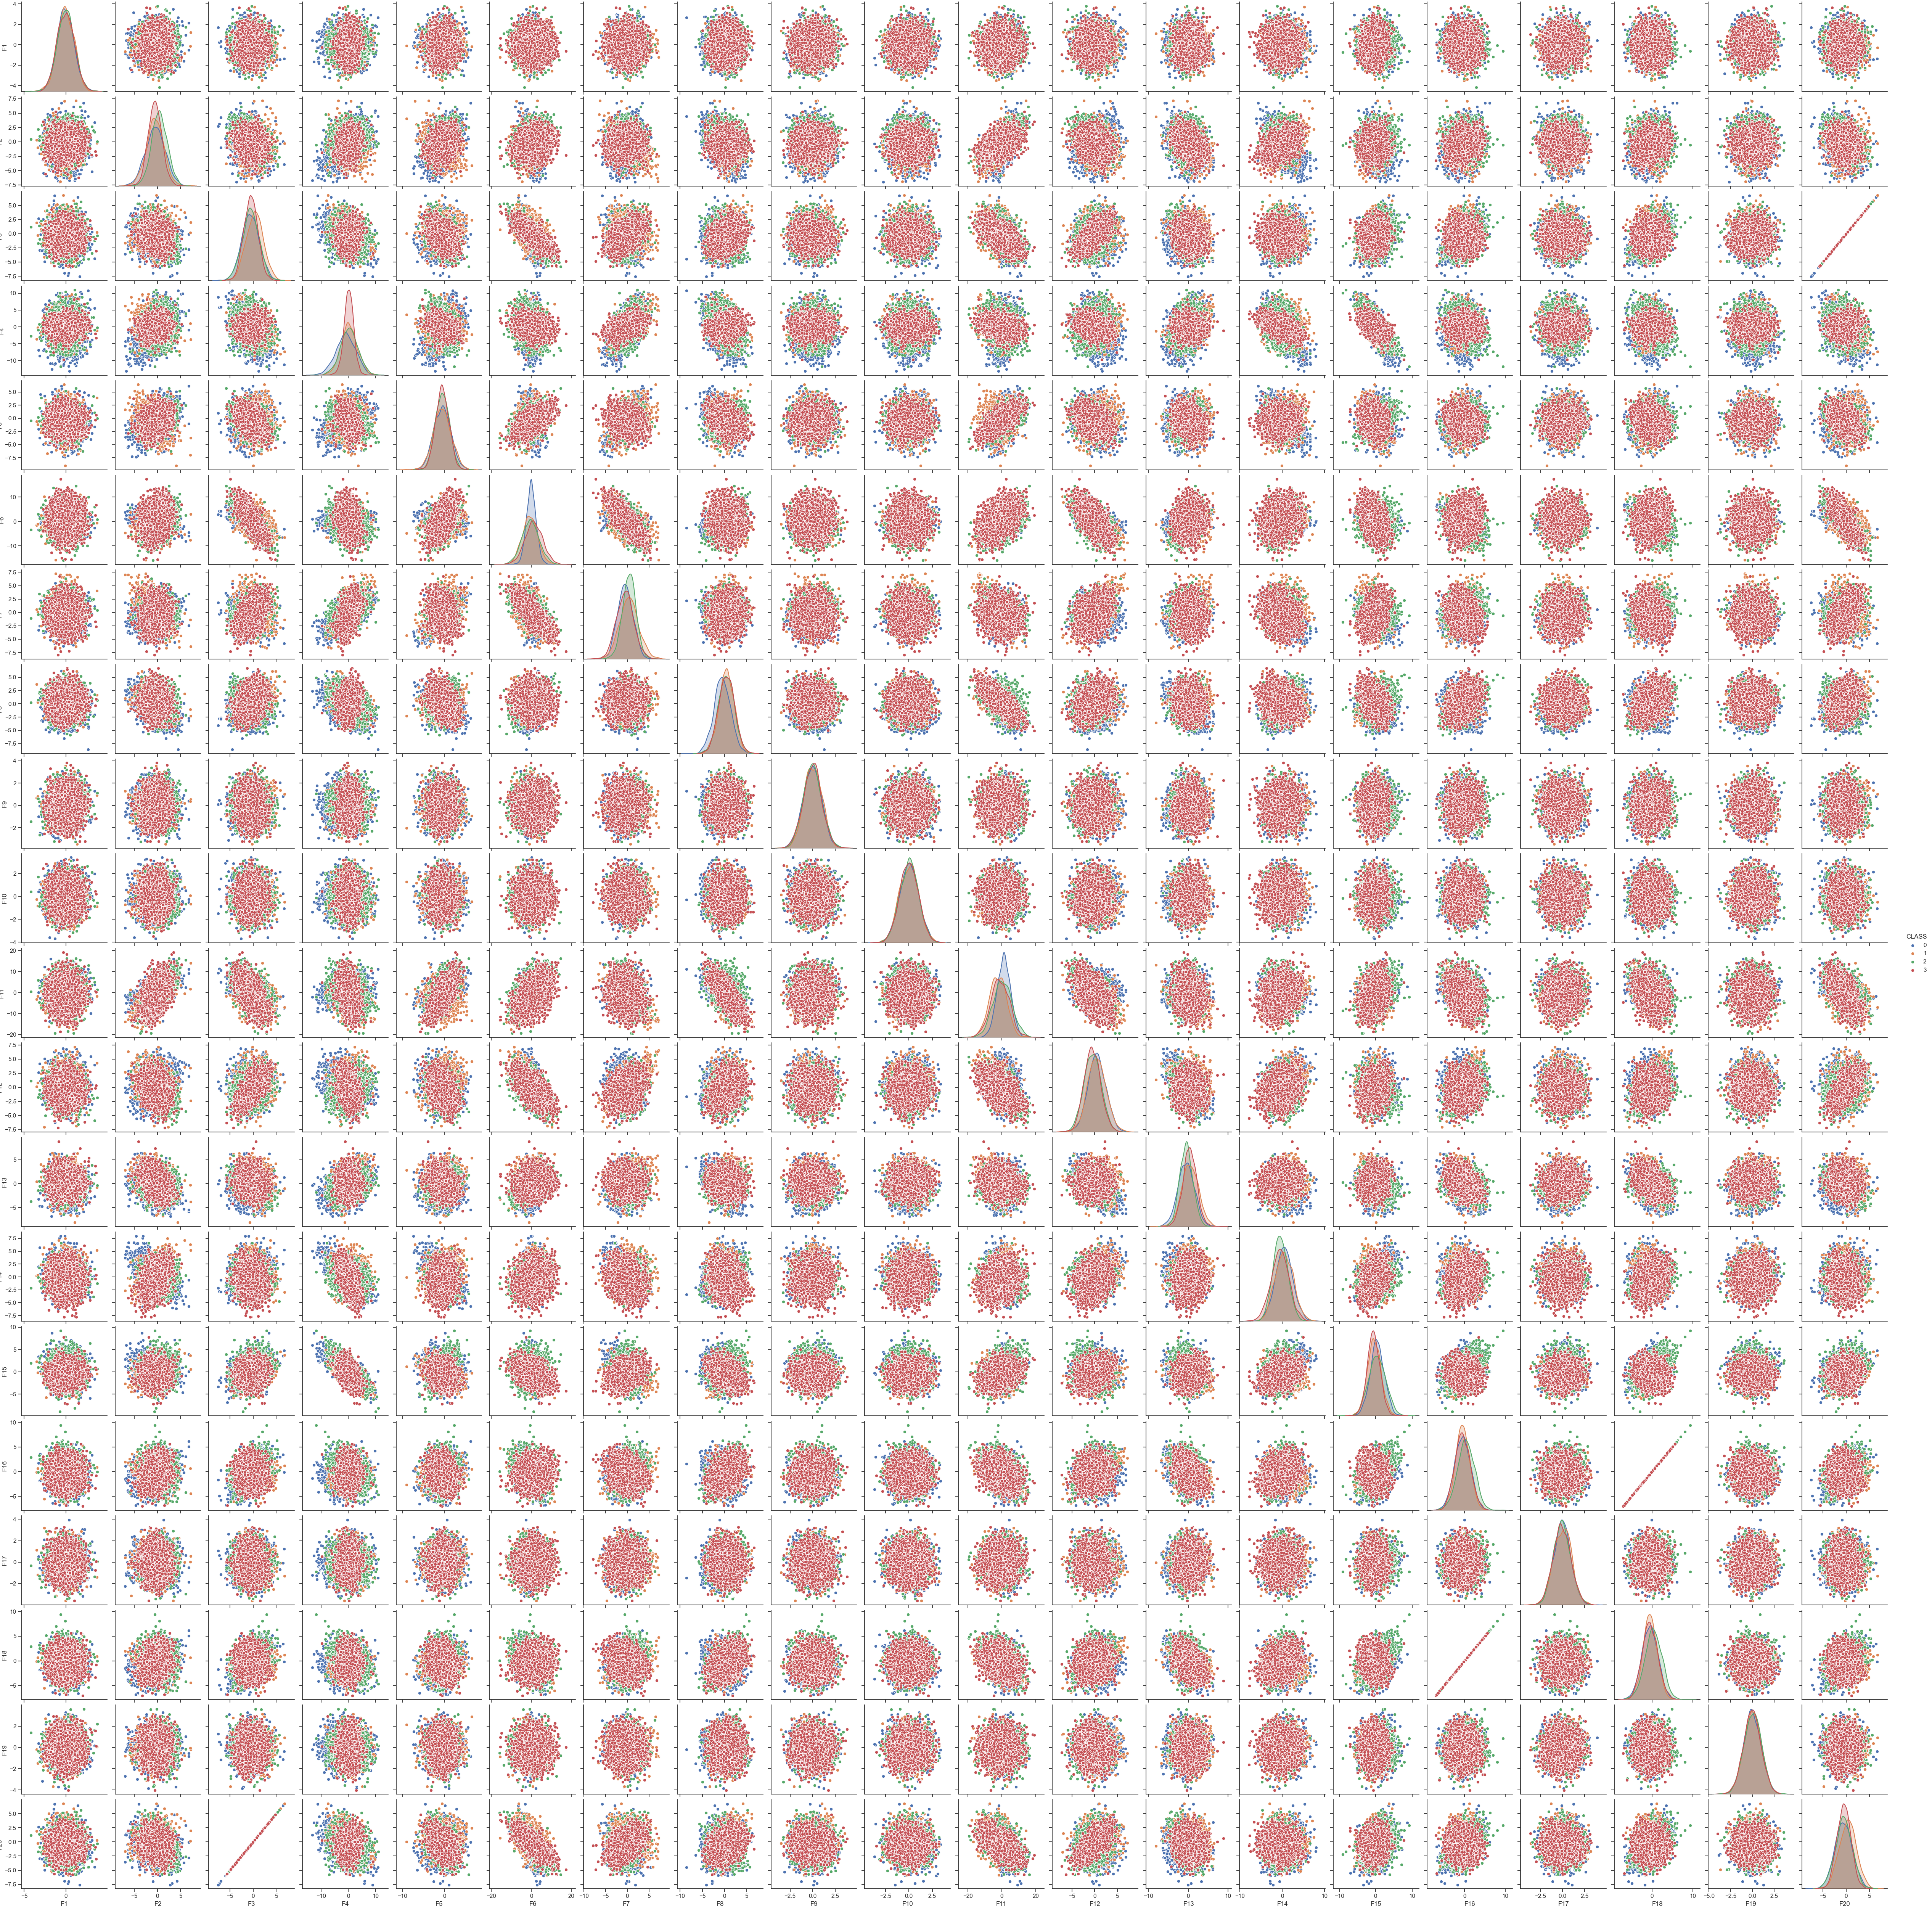
\includegraphics[width=175mm]{training_set}
                            \caption{Pair plot representing \textit{features}.}
                            \label{fig:training_set_pairplot}
                        \end{figure}
                        \clearpage
                
                \subsubsection{Data sampling} 
                
                        Il \textit{dataset} considerato presenta elementi così distribuiti:
                        \begin{itemize}
                                \item \textit{Class 1}: $33.67 \, \%$
                                \item \textit{Class 2}: $15.99 \, \%$
                                \item \textit{Class 3}: $20.66 \, \%$
                                \item \textit{Class 4}: $29.68 \, \%$
                        \end{itemize}
                        
                        \`E stato quindi effettuato balancing delle classi per evitare che il modello finale pecchi nel riconoscimento di classi meno presenti nel \textit{training set}.
                        
                        La tecnica di balancing utilizzata è lo \textit{SMOTE}.
                        
                        \textbf{TODO}
                

        \subsection{Hyper-parameters tuning}
        
                I modelli utilizzati per la classificazione sono:
                \begin{itemize}
                        \item \textit{Multi-Layer Perceptron}
                        \item \textit{Support Vector Machine}
                        \item \textit{Decition Tree}
                        \item \textit{Random Forest}
                        \item \textit{K-Nearest Neighbors}
                        \item \textit{Stochastic Gradient Descent}
                        \item \textit{Ada Boost}
                        \item \textit{Naive Bayes}
                        \item \textit{K-Means}
                \end{itemize}
            
                In questa fase sono stati cercati gli \textit{iper-parametri} migliori per i vari classificatori tra quelli elencati nella seguente tabella.
                
                \begin{center}
                	\begin{tabular}{+l^c^c}
                		\toprule\rowstyle{\bfseries}
                		Model & Parameters \\
                		\toprule
                		
                		Multi-Layer Perceptron & \makecell[l]{activation: [tanh, relu] \\ hidden\_layer\_sizes: [(150, 100), (120, 60), (60, 30), (75), (45)] \\ learning\_rate: [constant, adaptive] \\ learning\_rate\_init: [1e-1, 1e-2, 1e-3, 1e-4] \\ solver: [sgd, adam]}  \\
                		\midrule
						 Support Vector Machine & \makecell[l]{kernel: linear \\ C: [0.1, 1, 10] \\ decision\_function\_shape: [ovo, ovr]\\ \midrule kernel: rbf \\ C: [0.1, 1, 10] \\ decision\_function\_shape: [ovo, ovr] \\ gamma: [1e-4, 1e-3, 1e-2, 1e-1, 1e+1, 1e+2, 1e+3, 1e+4] \\
						 \midrule kernel: poly \\ C: [0.1, 1, 10] \\ degree: [2, 3, 4]\\ decision\_function\_shape: [ovo, ovr] \\ gamma: scale} \\
						 \midrule
						 Decision Tree & \makecell[l]{criterion: [entropy, gini] \\ max\_depth: [80, 90] \\ max\_features: [log2, sqrt, None] \\ min\_samples\_leaf: [2, 5, 10] \\ splitter: [best, random]} \\
						 \midrule
						 Random Forest & \makecell[l]{criterion: [entropy, gini] \\ max\_depth: [80, 90] \\ max\_features: [log2, sqrt, None] \\ min\_samples\_leaf: [2, 5, 10] \\ n\_estimators: [100, 200, 300, 400, 500]} \\
						 \midrule
						 K-Nearest Neighbors & \makecell[l]{metric: [minkowski, euclidean, chebyshev] \\ n\_neighbors: [3, 5, 7, 11] \\ p: [3, 4, 5]} \\
						 \midrule
						 Ada Boost &  \makecell[l]{criterion: [entropy, gini] \\ class\_weight: balanced \\ max\_depth: 90 \\ max\_features: 3 \\ min\_samples\_leaf: 4 \\ n\_estimators: [100, 200, 300]\\ splitter: [best, random]} \\
						 \midrule
						 Naive Bayes & \makecell[l]{priors: [None, [0.25, 0.25, 0.25, 0.25]] \\ var\_smoothing: [10e-9, 10e-6, 10e-3, 10e-1]} \\
						 \midrule
						 K-Means & \makecell[l]{max\_iter: 10000 \\ n\_clusters: 4 }\\
 
                		\toprule\rowstyle{\bfseries}
                	\end{tabular}
                	\captionof{table}{Lista degli iperparametri testati per ogni modello di \textit{machine learning} testati}
                	\label{tab:f1scoreML}
                \end{center}
                

        \subsection{Evaluation}
        
                La metrica utilizzata al fine della valutazione dei classificatori è la \textit{f1-score} (media armonica), definita come segue:
                \begin{displaymath}
                F1 = \frac{2 \cdot precision \cdot recall}{precision + recall}
                \end{displaymath}
                con,
                \begin{displaymath}
                precision = \frac{TP}{TP + FP} \qquad recall = \frac{TP}{TP + FN}
                \end{displaymath}
                essendo $TN$ il numero di veri negativi, $FP$ il numero di falsi positivi, $FN$, falsi negativi e $TP$ veri positivi.